\documentclass[12pt,a4paper]{article}
\usepackage[utf8]{inputenc}
\usepackage[T1]{fontenc}
\usepackage[brazil]{babel}
\usepackage[a4paper,margin=2.5cm]{geometry}
\usepackage{graphicx}
\usepackage{booktabs}
\usepackage{amsmath}
\usepackage{float}
\usepackage[round,authoryear]{natbib}
\usepackage[hidelinks]{hyperref}
\graphicspath{{../outputs/figures/}}
\setlength{\parskip}{0.4em}
\renewcommand{\arraystretch}{1.15}

\title{\textbf{Previsibilidade da exposição das gestoras a ações} \\[0.4em]
\large Resultados de forecasting --- documento complementar ao TCC}
\author{João Paulo Zangrandi \\ \small Orientador: Prof.\ Maurício Ferraresi Junior --- FGV EESP}
\date{\today}

\begin{document}

\begin{titlepage}
\centering
\vspace*{1.5cm}
{\scshape\large Fundação Getulio Vargas --- EESP\par}
\vspace{2.5cm}
{\huge\bfseries Previsibilidade da exposição das gestoras a ações\par}
\vspace{0.6cm}
{\Large Cinco rodadas de forecasting \emph{out-of-sample} (2016--2021)\par}
\vspace{3cm}
{\Large João Paulo Zangrandi\par}
\vspace{0.4cm}
{\large Orientador: Prof.\ Maurício Ferraresi Junior\par}
\vfill
{\large São Paulo --- \today\par}
\end{titlepage}

\section*{Resumo}
\addcontentsline{toc}{section}{Resumo}
Investigamos se a exposição das gestoras a ações é \emph{previsível}, com avaliação \emph{out-of-sample}
(origem móvel, sem vazamento) e o \emph{random walk} (RW) como referência. Os resultados, em cinco rodadas:
(i)~a \textbf{variação mensal} da posição é \textbf{imprevisível} --- nenhum modelo bate o RW e a direção é
um cara-ou-coroa (50,8\%); (ii)~o \textbf{nível} da posição (em ITUB4) é previsível por \textbf{reversão à
média} (o AR bate o RW em $\sim$10\%), mas o peso não; (iii)~\textbf{features de rede} (exposição dos
vizinhos no grafo fundo-sobre-fundo) \textbf{não acrescentam} sinal ($\gamma\approx0$), o que torna um GNN
improvável de ajudar a \emph{prever}; (iv)~ao generalizar para 238 ações, a previsibilidade do nível
\textbf{não é geral}: concentra-se nas \emph{blue chips} muito detidas (ITUB4 está entre as 3 mais
previsíveis), enquanto para a ação típica o RW vence. A leitura econômica: a demanda institucional é em larga
medida imprevisível; o componente previsível é a \emph{alocação-alvo estável} nos papéis mais concentrados ---
exatamente onde também se concentra a fragilidade de \citet{greenwoodthesmar2011}.

\newpage
\tableofcontents
\newpage

\section{Desenho da avaliação}\label{sec:setup}
\textbf{Alvo.} Seguindo o orientador, partimos da \emph{variação mensal} da posição em US\$ de cada gestora,
$\Delta\text{pos}_{g,t}$; depois testamos o \emph{nível} $\text{pos}_{g,t}$ e o peso.
\textbf{Avaliação.} Origem móvel com janela expansível: treina-se em $1..t$ e prevê-se $t{+}h$, começando após
36 meses. Tudo \emph{out-of-sample} e \textbf{sem vazamento} (PCA, fatores e coeficientes estimados só no
treino). \textbf{Referência:} \emph{random walk} --- para a variação, $\widehat{\Delta}=0$; para o nível,
$\widehat{y}_{t+h}=y_t$. \textbf{Métricas:} RMSE e MAE (\emph{skill} $=$ \% de redução de erro vs RW), acerto
de direção (vs 50\%) e testes pareados.

\section{A variação mensal é imprevisível}\label{sec:var}
A Tabela~\ref{tab:r12} resume as rodadas 1--2 (alvo $\Delta$pos US\$). \textbf{Nenhum modelo bate o RW}: o AR
fica $-1\%$, a média $-1{,}3\%$ e o fator-PCA \emph{piora} (até $-14\%$). Encolher o AR em direção ao ``não
muda'' (RW) dá um ganho trivial de $+1\%$ em RMSE. O \textbf{acerto de direção} (subir/descer) chega a no
máximo 50,8\% --- estatisticamente um \textbf{cara-ou-coroa} ($p=0{,}59$). Nota metodológica: o PCA piora
\emph{mais} quanto mais fatores ($k{=}1$ melhor que $k{=}3$), o sinal clássico de \emph{overfitting} em
janelas curtas.

\begin{table}[H]\centering
\caption{Variação mensal da posição (US\$): \emph{skill} vs random walk e acerto de direção.}
\label{tab:r12}
\small
\begin{tabular}{lrrr}
\toprule
\textbf{Modelo} & \textbf{Skill RMSE} & \textbf{Skill MAE} & \textbf{Acerto direção} \\
\midrule
Random walk ($\widehat{\Delta}=0$) & 0,0\%  & 0,0\%   & --- \\
AR encolhido ($0{,}5\cdot$AR)       & $+1{,}0\%$ & $-1{,}8\%$ & 47,8\% \\
AR($p$)                             & $-1{,}0\%$ & $-6{,}3\%$ & 47,8\% \\
PCA fatorial ($k{=}1$)              & $-2{,}8\%$ & $-8{,}6\%$ & 48,2\% \\
PCA fatorial ($k{=}3$)              & $-14{,}1\%$ & $-23{,}0\%$ & 50,8\% \\
\bottomrule
\end{tabular}
\end{table}

\section{O nível reverte à média (e é previsível)}\label{sec:nivel}
Mudando o alvo para o \emph{nível} da posição (Tabela~\ref{tab:r3}, Figura~\ref{fig:r3}), surge
previsibilidade: para ITUB4, o AR bate o RW em \textbf{$+10\%$} (h$=$1 e 3) e o modelo de painel com
reversão à média melhora com o horizonte ($+9\%$ em 6 meses). Economicamente: gestoras têm uma
\textbf{exposição-alvo} à qual retornam. O \textbf{peso}, porém, comporta-se como \emph{random walk} (o AR
perde em todos os horizontes) --- nuance ao palpite de que o peso seria ``mais estacionário''.

\begin{table}[H]\centering
\caption{Previsão do NÍVEL: \emph{skill} vs RW (\%), por alvo e horizonte (ITUB4).}
\label{tab:r3}
\small
\begin{tabular}{llrrr}
\toprule
\textbf{Alvo} & \textbf{Modelo} & \textbf{h$=$1} & \textbf{h$=$3} & \textbf{h$=$6} \\
\midrule
Posição US\$ & AR individual & $+10{,}0$ & $+10{,}2$ & $+7{,}1$ \\
Posição US\$ & AR painel     & $+3{,}3$  & $+7{,}8$  & $+9{,}0$ \\
Peso         & AR individual & $-11{,}4$ & $-16{,}8$ & $-25{,}5$ \\
Peso         & AR painel     & $-4{,}0$  & $-14{,}8$ & $-26{,}0$ \\
\bottomrule
\end{tabular}
\end{table}

\begin{figure}[H]\centering
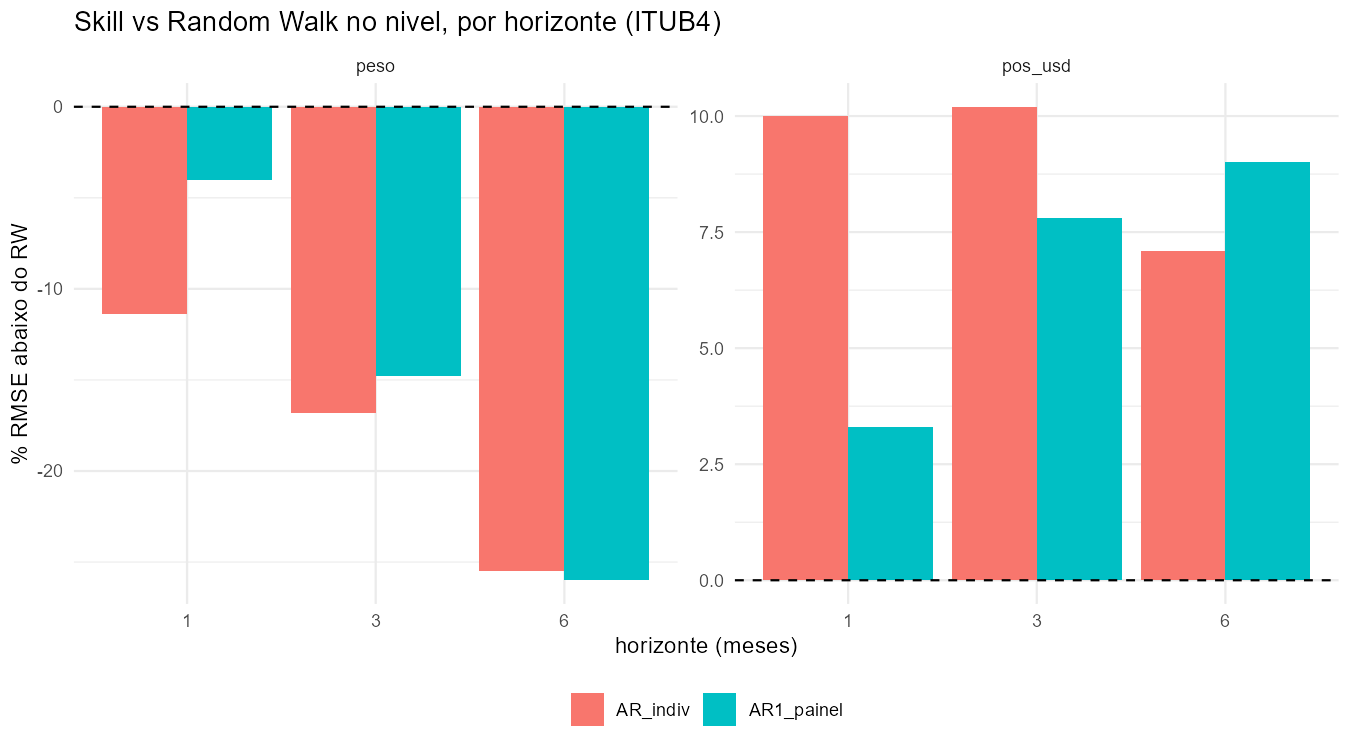
\includegraphics[width=0.85\textwidth]{forecast_round3_skill.png}
\caption{\emph{Skill} vs random walk no nível, por horizonte. Posição US\$ (esq.) é previsível; peso (dir.) não.}
\label{fig:r3}
\end{figure}

\section{A rede não ajuda a prever}\label{sec:rede}
Adicionamos ao modelo de nível um preditor de \textbf{rede}: a exposição (defasada) das gestoras
\emph{vizinhas} no grafo fundo-sobre-fundo (ligações cross-gestora via FICs). O coeficiente de rede é
$\gamma\approx0{,}01$ (praticamente zero) e o \emph{skill} \emph{não} melhora ($+3{,}1\%$ com rede vs
$+3{,}3\%$ sem). Ou seja, a previsibilidade é \textbf{idiossincrática} (reversão à média própria), não
contágio pela rede. \textbf{Implicação prática:} como \emph{features} de rede feitas à mão não acrescentam,
um \textbf{GNN} --- que aprende da mesma estrutura --- é improvável de ajudar a \emph{prever}. O valor da rede
é \textbf{descritivo} (medir o risco: a dupla contagem fundo-sobre-fundo de 37\%), não preditivo.

\section{A previsibilidade não generaliza --- concentra-se nas \emph{blue chips}}\label{sec:geral}
Repetindo o forecast de nível para \textbf{238 ações} com histórico suficiente (Figura~\ref{fig:r5}): a
\emph{skill} mediana é \textbf{$-13{,}5\%$} e apenas \textbf{10\%} das ações batem o RW. Mas \textbf{ITUB4
está entre as 3 mais previsíveis} ($+9{,}9\%$), ao lado de PETR3 ($+9{,}7\%$) e ITSA4 ($+9{,}6\%$) --- todas
\emph{blue chips} detidas por quase todas as gestoras. \textbf{ITUB4 não era representativo: era um dos casos
mais favoráveis.} A previsibilidade por reversão à média existe onde as gestoras mantêm \textbf{alocações-alvo
estáveis} (papéis líquidos e \emph{crowded}); para a ação típica, de posição intermitente, o random walk
vence. (Excluímos $\sim$5 séries degeneradas por troca de \emph{ticker}/\emph{delisting}, p.ex.\ BVMF3$\to$B3SA3.)

\begin{figure}[H]\centering
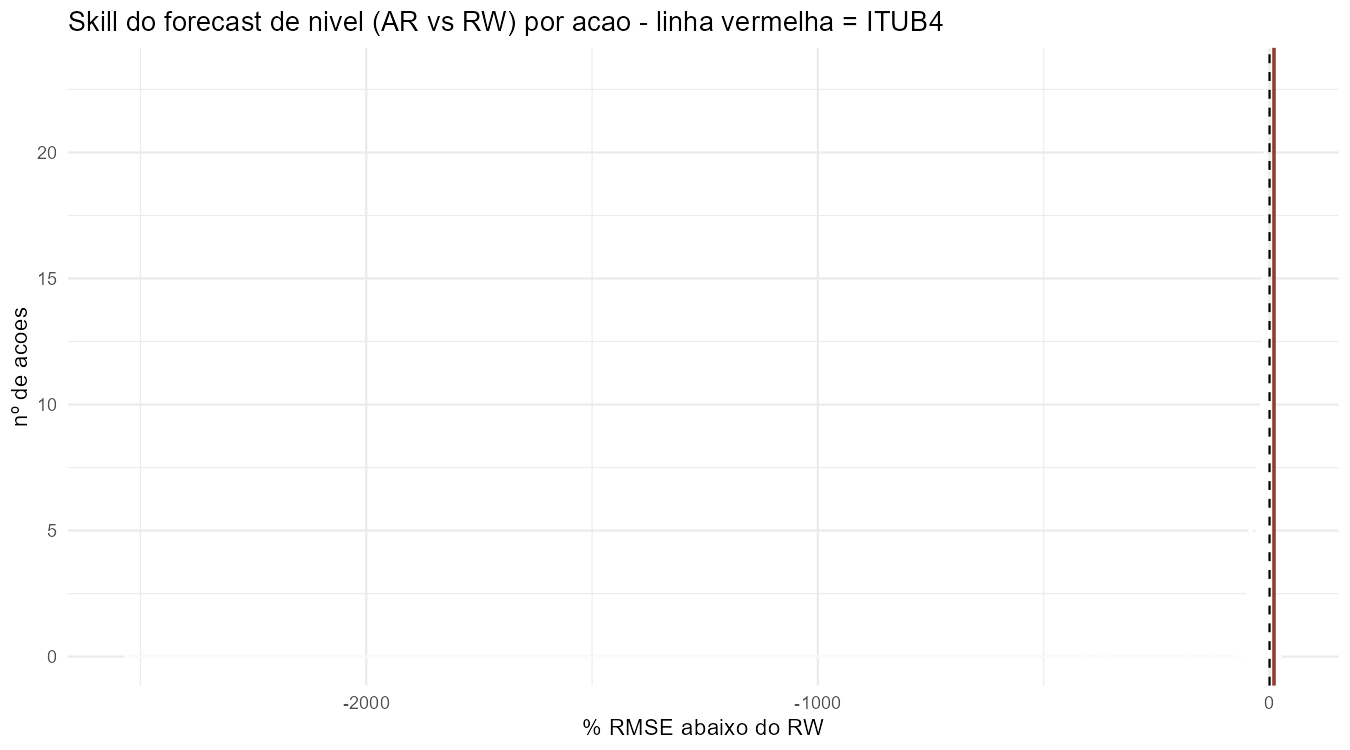
\includegraphics[width=0.85\textwidth]{forecast_round5_skill_hist.png}
\caption{Distribuição da \emph{skill} (AR vs RW) entre 238 ações. Linha vermelha $=$ ITUB4 (entre as melhores).}
\label{fig:r5}
\end{figure}

\section{Discussão}\label{sec:disc}
Os resultados desenham um quadro coerente com \emph{demand-based asset pricing}
\citep{koijenyogo2019,gabaixkoijen2021}: a demanda institucional muda de forma \textbf{quase imprevisível} no
curto prazo (variação mensal $\approx$ martingale), e o que há de previsível é a \textbf{reversão a uma
alocação-alvo}, concentrada justamente nas ações mais \emph{crowded}. Isso é duplamente relevante: são esses
papéis que (a)~concentram demanda institucional sobreposta e (b)~são mais \emph{frágeis} no sentido de
\citet{greenwoodthesmar2011}. Em outras palavras, onde a demanda é previsível é também onde o risco de
co-movimento é maior. Por fim, a rede fundo-sobre-fundo é \textbf{essencial para medir o risco}
(de-duplicação, estruturas aninhadas) mas \textbf{não para prever} a exposição --- por isso não levamos o GNN
adiante para forecasting.

\section{Limitações e próximos passos}\label{sec:lim}
Painel curto (72 meses) e frequência mensal limitam a potência dos testes; a validação é centrada em ITUB4 e
nas \emph{blue chips}; séries com troca de \emph{ticker} foram excluídas. Caminhos: horizontes/frequências
alternativas; modelar a \emph{alocação-alvo} explicitamente (correção de erro/half-life de reversão);
e, no eixo de \emph{risco} (não de previsão), aprofundar as métricas de rede (ciclos, profundidade, peso
indireto) já disponíveis. O arcabouço de avaliação (\texttt{R/13}--\texttt{R/17}) é reutilizável para todas as
ações.

\bibliographystyle{plainnat}
\bibliography{refs}
\end{document}
